Before we can perform any kind of feature extraction over the 3D shapes, we first have to prepare our data set so that the shapes are resampled and normalized.
We want all the shapes in our data set to have approximately the same number of faces and vertices.
The reasoning behind this is that in the feature extraction step, we would like to compute fixed-size feature vectors
using local descriptors, and allowing for shapes that differ by orders of magnitude in the number of vertices and
number of faces might lead to inaccurate features between different shapes.
Aside from the same number of faces and vertices, we would also like to compute features that are invariant with
respect to the rotation or scale of a shape.
In order to achieve this we transform the data set shapes such that after a series of such transformations all the
shapes have the following properties:
\begin{itemize}
    \item the barycenter of the shape is in the origin of the coordinate space;
    \item the shapes are re-scaled to the unit cube;
    \item the shapes are aligned such that the most spread of the shape is along the $x$ coordinate axis, the medium spread is aligned along the $y$-axis and the minimal spread is aligned along the $z$-axis;
    \item the shape is concentrated on the positive side of each plane $x = 0, y = 0, z = 0 $. 
\end{itemize}


\subsection{Analysing a Single Shape}
The preprocessing step involves getting certain information about the shapes, detecting the ones which are not
quality-compliant, and then preprocessing them in such a way that they fit our requirements.
This section will discuss our approach to doing this.

For the preprocessing stage, the information we track for each shape is the number of vertices, number of faces, the
type of faces (triangles/squares/mixed), and the axis-aligned bounding box of the shape.

Getting this information is largely done via methods that are already implemented in PyMeshLab.
The number of vertices and faces are accessed with the \verb!vertex_number()! and \verb!face_number()! methods
respectively.
The type of faces for a given shape is determined by the number of points $p$ in a face $f = (p_1, ..., p_n)$ belonging to the set of faces \ref{faces_not}.
If, for all $f \in$ \ref{faces_not}; $n = 3$, the shape is constructed of triangles;
if $n = 4$ for all $f \in$ \ref{faces_not}, the shape is constructed of quads (rectangular polygons);
if some $n = 3$ and some $n = 4$, then it is a mixed shape.
The bounding box is extracted via the \verb!bounding_box()! method, and then aligned along each dimension $x, y, z$ and the diagonal of the shape.

Two examples of the output of this analysis and the respective visualisations of the shape are shown in Figure
\ref{fig:analysed}.
The shapes we chose are the two that have a number of faces and vertices which is closest to the respective average
in the dataset.
Notice that the number of vertices, faces, their type, and the coordinates of the bounding box are shown below the meshes.

\begin{figure}[ht]
    \centering
    \begin{subfigure}{0.45\textwidth}
        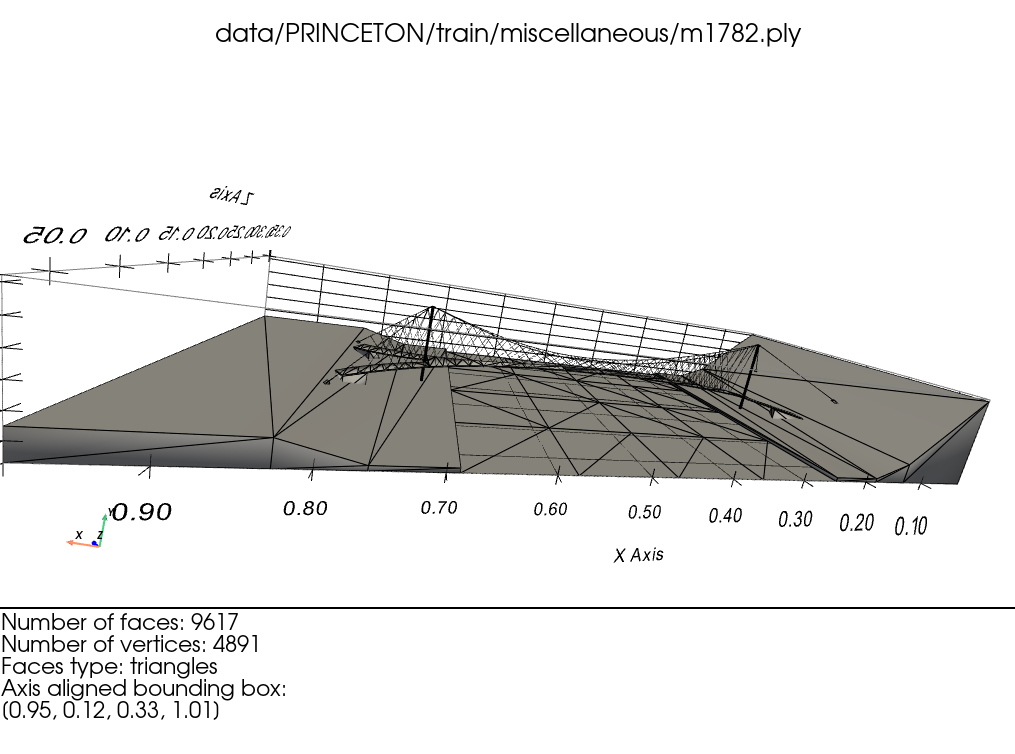
\includegraphics[width=\textwidth]
        {assets/visualisation/faces_avg_shape.png}
        \caption{Model with number of faces closest to the average number of faces}
    \end{subfigure}
    \hfill
    \begin{subfigure}{0.45\textwidth}
        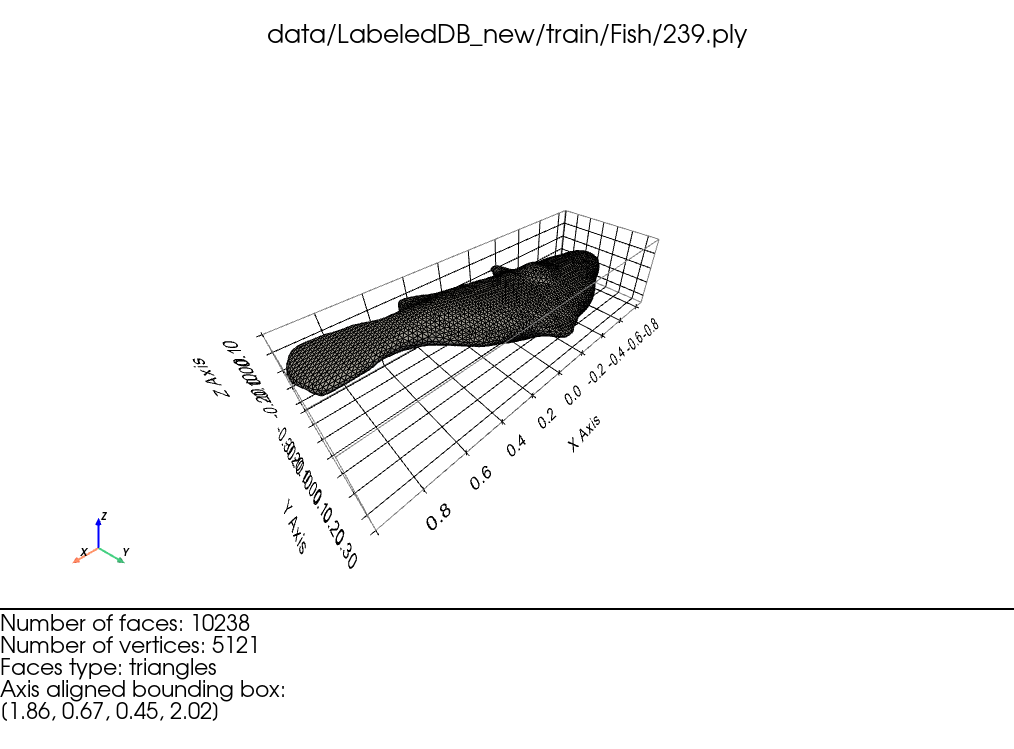
\includegraphics[width=\textwidth]
        {assets/visualisation/vertices_avg_shape.png}
        \caption{Model with number of vertices closest to the average number of vertices}
    \end{subfigure}
    \caption{Visualisation with the number of vertices, number of faces, faces type and the bounding box computed.}
    \label{fig:analysed}
\end{figure}

\subsection{Statistics Over the Whole Database}
As we will see in one of the following subsections, the normalisation process does not require any decisions or user-defined parameters.
This is not the case however in the resampling step, where we have to decide on a few variables.
One of these is the number of faces (or, by proxy, number of vertices) we want the shapes in our database to be made up of.
This subsection presents statistics about our data set along with reasoning for the design choices we made in creating the resampling process.

In order to understand our dataset, we first perform a class distribution analysis in which we compute the distribution of the shapes in the data set over the class labels.
The results are presented in Figure \ref{fig:class-distribution}.
Observe that the shapes are not uniformly distributed.
For instance, we have 200 objects in the vehicle class and only 20 in classes like Bust, Hand, Bird, etc.
However, this is not a problem for the system we develop.


In Figure \ref{fig:statistics-faces-vertices-number} we present the distribution over the number of faces and number of vertices of the shapes.

Since we would like to make our system independent of the data set and, more importantly, we would like our system to work quickly, we decided to resample the shapes such that, for each shape \ref{shape_not}, \ref{faces_not}=5000.
In choosing the value for this number, we considered firstly what it will be used for - computing descriptive features of the shapes.
A higher value gives more accurate results, but requires (much) more computation.
For many features, the $\mathcal{O}$ computation is dependant, in some way, on the number of \ref{faces_not}.
However, having a value that is too low would result in features which are very inaccurate for the original shape that we are trying to describe.
$5000$ is a good compromise between these two factors, as well as a good heuristic approximation to the usual number of faces we believe a 3D shape will have.

\begin{figure}
    \centering
    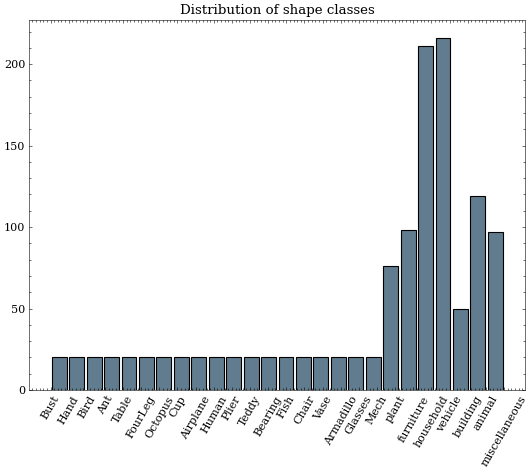
\includegraphics[width = 0.8\textwidth]{assets/preprocessing/Distribution_of_shape_classes.png}
    \caption{Distribution of shape classes}
    \label{fig:class-distribution}
\end{figure} 

\begin{figure}
    \centering
    \begin{subfigure}[b]{0.45\textwidth}
         \centering
         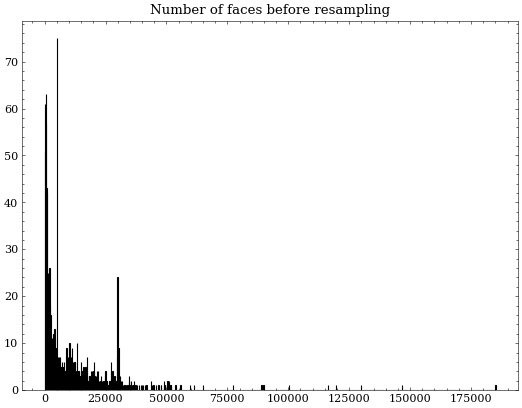
\includegraphics[width=\textwidth]{assets/preprocessing/Number_of_faces_before_resampling.png}
         \caption{Distribution of the number of faces}
         \label{fig:statistics-faces-vertices-number-a}
     \end{subfigure}
     \hfill
     \begin{subfigure}[b]{0.45\textwidth}
         \centering
         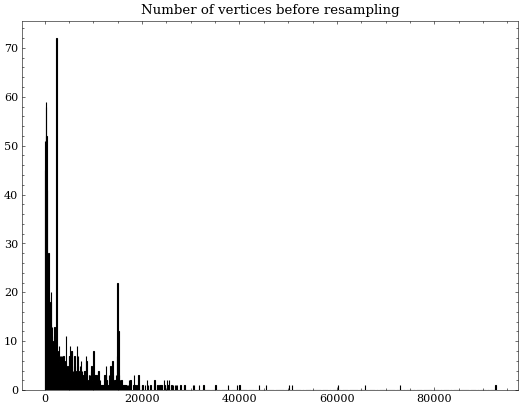
\includegraphics[width=\textwidth]{assets/preprocessing/Number_of_vertices_before_resampling.png}
         \caption{Distribution of the number of vertices}
         \label{fig:statistics-faces-vertices-number-b}
     \end{subfigure}
    \caption{Statistics for resampling decisions}
    \label{fig:statistics-faces-vertices-number}
\end{figure}

\subsection{Sub-Sampling and Super-sampling}
The 3D meshes of the shapes we are working with have a different number of faces and vertices, as can be seen in
Figure \ref{fig:statistics-faces-vertices-number}.
In order to compare these shapes with each other fairly, we first have to manipulate these meshes such that these
amounts are roughly the same between shapes.
That way, the features that will eventually be extracted, will be meaningful to us and our shape retrieval system -
at the end of the day, we want to compare the shapes to each-other, and that can only be done fairly if they have a
similar granularity.
As we mentioned earlier, we have chosen to resample the meshes such that the number of faces comes near the predefined
number of $5000$ faces.
If shapes have a higher number of faces, then we have to lower this amount.
Whenever the amount of faces is very low compared to $5000$, then we have to somehow increase the number of faces.
This is done by respectively sub-sampling and super-sampling the 3D meshes.
In this subsection we explain how exactly we implemented this.

As discussed in our environment setup, PyMeshLab offers extensive functionality for performing operations on meshes.
It offers a wide range of so-called filters for many tasks, such as mesh manipulation and processing.
Among these filters, there is a selection of several algorithms which can be used for re-meshing 3D meshes.

\paragraph{Sub-sampling}
For sub-sampling, we use the following configuration:
\begin{itemize}
    \item the ``Meshing Decimation Quadric Edge Collapse'' filter. This filter simplifies the mesh to a mesh with a
    specific target amount of faces lower than the original amount of faces;
    \item a target amount of faces, which we have set to $5000$, the wanted amount of faces;
    \item a quality threshold of $1$, which is the other parameter for this filter. This value penalizes bad shaped faces maximally. Thus, we try to keep the original surface of the shape as intact as possible.
\end{itemize}

In Figure \ref{fig:resampled_woman}, an example of the sub-sampling results is shown.
In it, we compare the original mesh of a model of a woman to its processed, sub-sampled, mesh.
Very detailed parts of the 3D model - such as the face, shoes, legs and hands, lose a lot of information, but they
still maintain the overall shape of the original mesh in those specific parts.
The areas of the resulting faces are also very comparable after sub-sampling, whereas the faces in the original mesh
had faces of varying sizes.
In fine-grained areas, such as the shoes of the model, there were some very small faces, while the dress for example
has faces with a fairly large area in comparison to those.
Again, this is to be expected, since more triangles are needed to model the finer details of the models.

\begin{figure}[ht]
  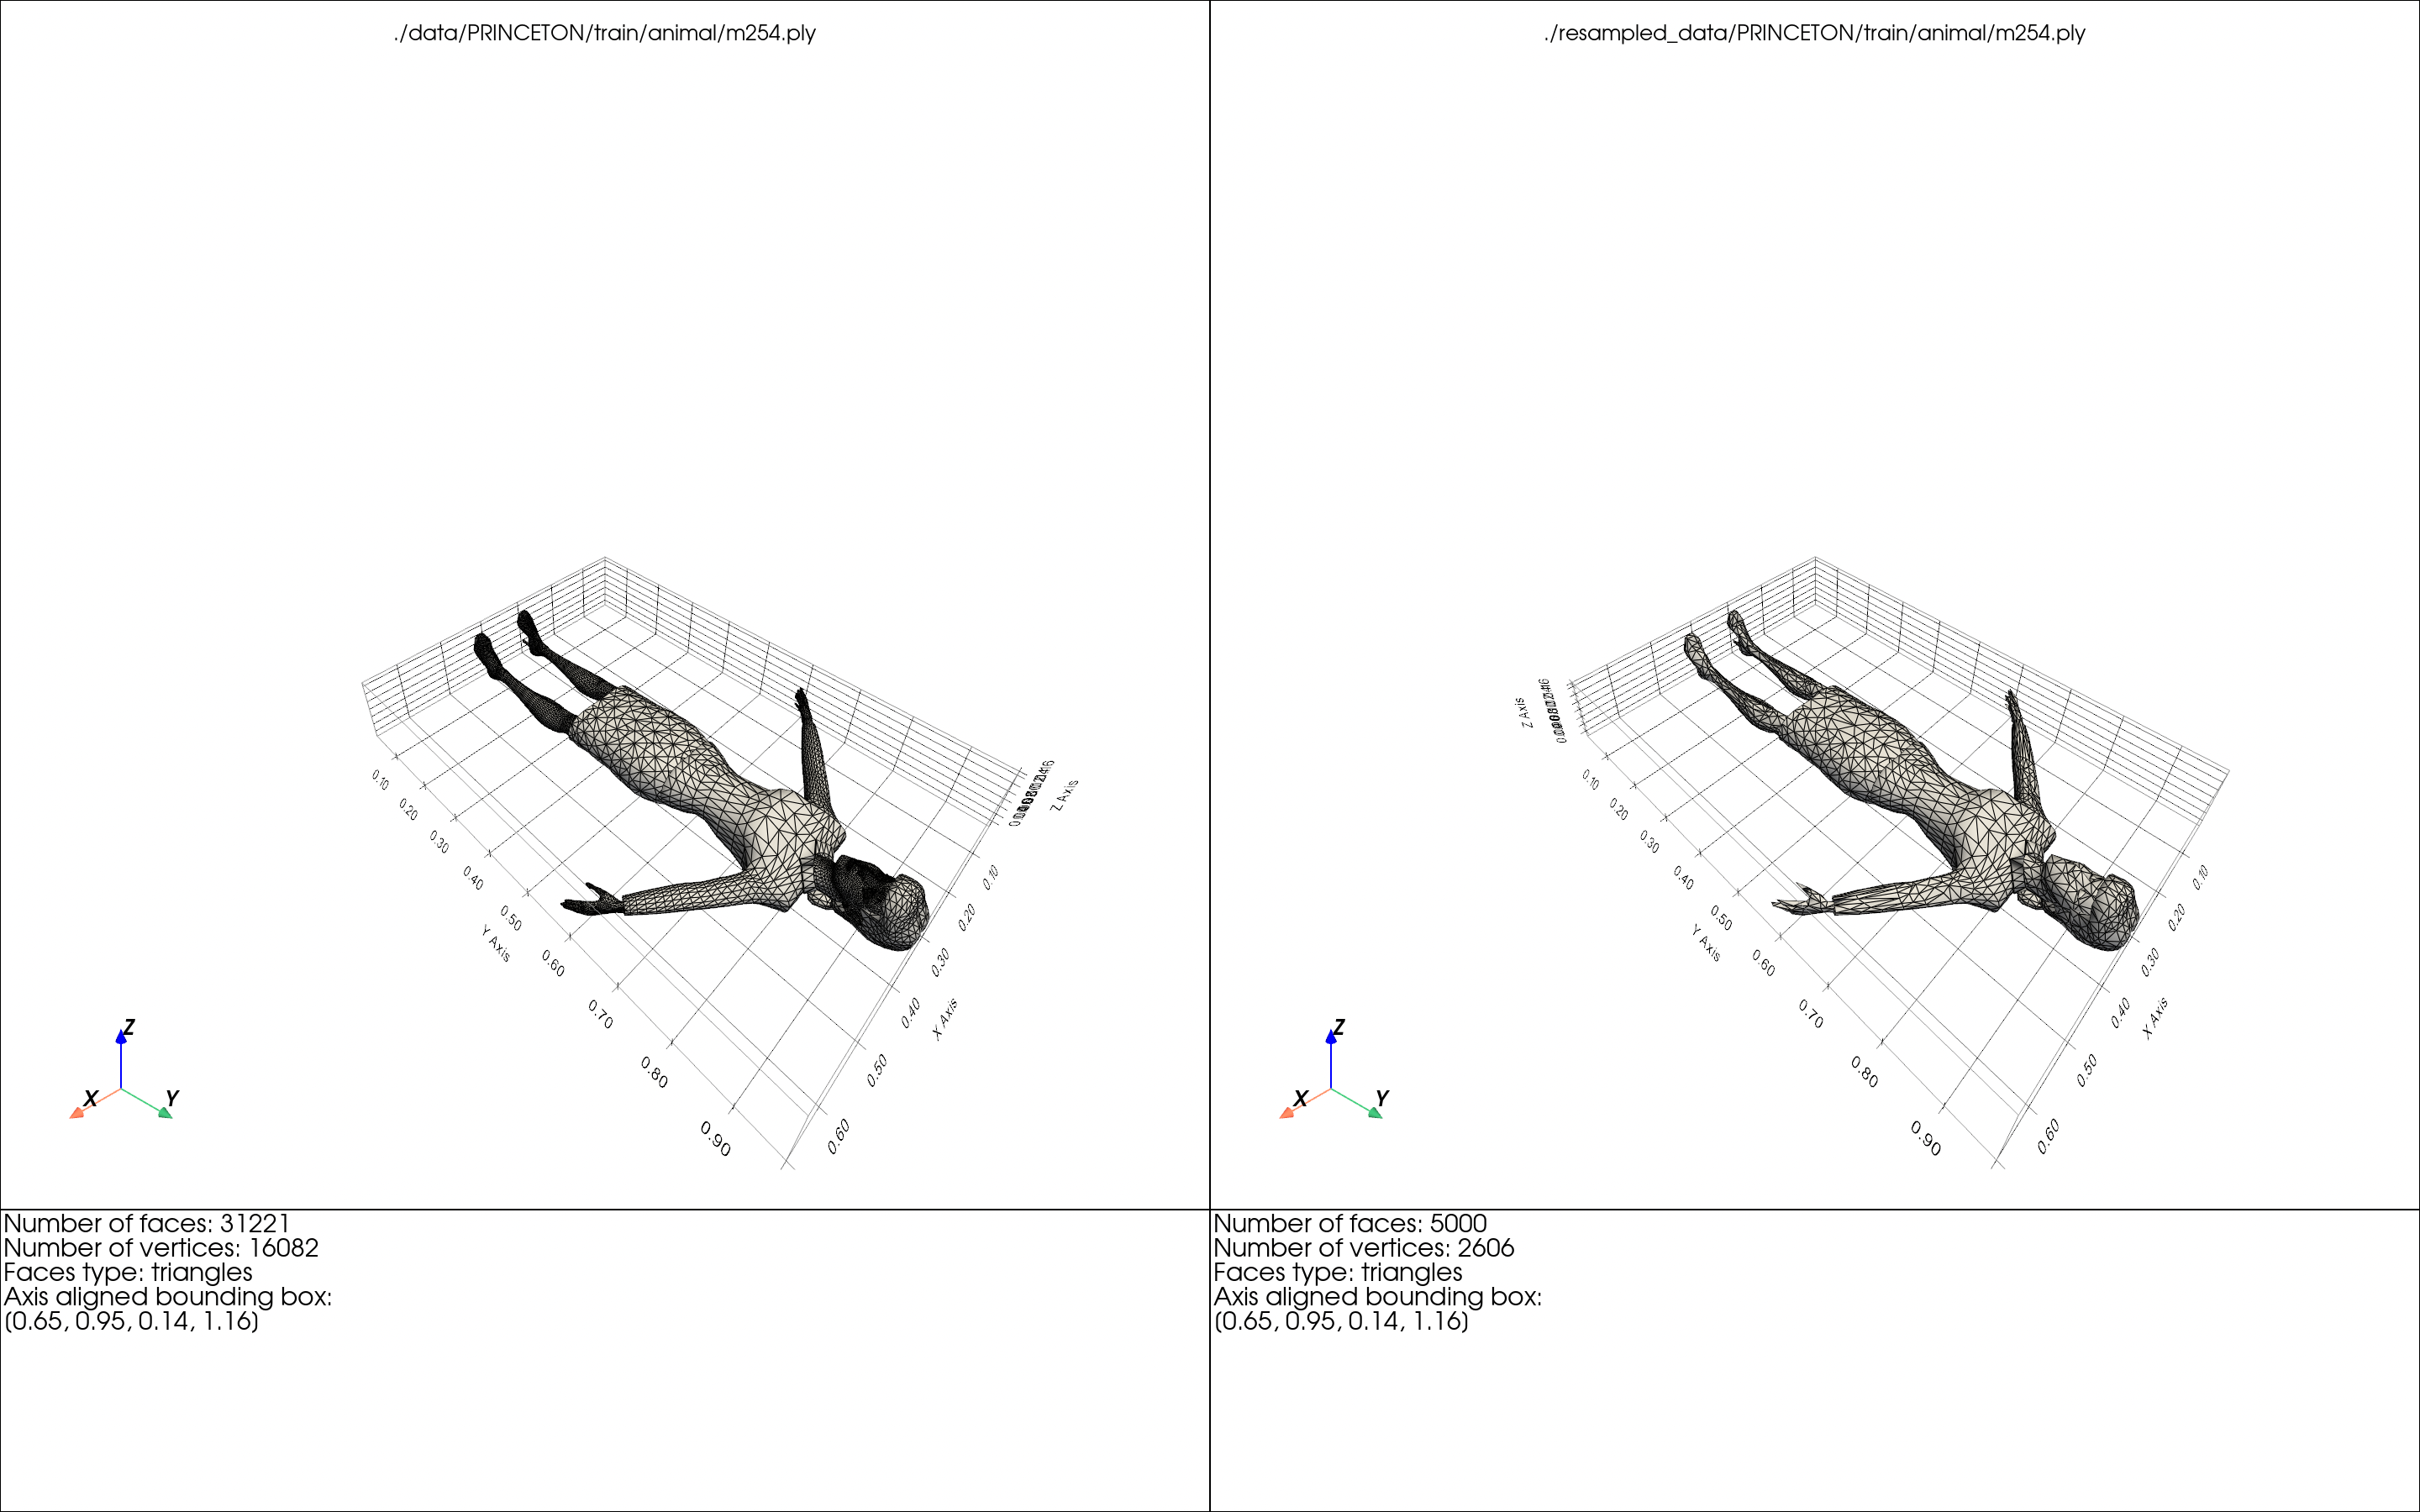
\includegraphics[width=\linewidth]
  {assets/preprocessing/resampling/woman_resampled.png}
  \caption{Comparison of the original 3D mesh of a woman on the left with its resulting sub-sampled mesh on the right.}
  \label{fig:resampled_woman}
\end{figure}

\paragraph{Super-sampling}
When we have to perform super-sampling on a mesh with a low number of faces, we are currently using the ``Meshing
Surface Subdivision Midpoint'' filter.
This filter splits each edge on its midpoint, creating a new set of faces, each of which is constructed in the
interior of the original face.
Since our database consists of 3D meshes that only have triangles as faces, every triangle face is replaced by the four triangle faces that can be formed in its interior.
Thus, every iteration of this algorithm multiplies the number of faces of the model by $4$.
Knowing this, we can calculate the exact number of iterations needed to reach (at least) the target amount of $5000$
faces.
This proves very useful as one of the required parameters for the subdivision algorithm implementation in PyMeshLab is
the number of iterations.
The implementation of super-sampling using this filter is somewhat more involved than for the sub-sampling.
The pipeline for our super-sampling implementation is as follows:
\renewcommand{\labelenumii}{\theenumii}
\renewcommand{\theenumii}{\theenumi.\arabic{enumii}.}
\begin{enumerate}
    \item Perform the subdivision algorithm to reach $5000$ or more faces, given the number of iterations needed.
    \item If the algorithm raises an error:
    \begin{enumerate}
        \item Try to repair the mesh with the ``Meshing Repair Non-Manifold Edges'' filter.
        \item If the repair is successful, try to perform the subdivision algorithm on the repaired mesh.
    \end{enumerate} 
    \item If the number of faces exceeds the wanted amount of faces, call the sub-sampling functionality described
    above to achieve exactly the target number of faces.
\end{enumerate}

%We provide this iteration amount as an argument to the filter to obtain a mesh with $5000$ faces or more. If the amount of faces exceeds $5000$ we use the sub-sampling to make sure that the target amount of faces is exactly $5000$.
As seen in step 2 of the workflow, the subdivision algorithm might fail if a mesh is not 2-manifold, i.e.\ if it
contains holes.
To account for this, we have implemented functionality that attempts to repair the mesh.
If the mesh is successfully repaired, we try to run the subdivision algorithm on the repaired mesh as necessary.
For the repairing of a mesh, we use the ``Meshing Repair Non-Manifold Edges'' filter.
Using this filter, we have the option of either removing the smallest area faces until the mesh becomes 2-manifold,
or splitting vertices in such a way that each non-manifold edge-chain will become a border.
The default behavior is to remove the faces with the smallest area, which is what we chose.
Finally, after the super-sampling is performed, we re-use the sub-sampling implementation to get meshes with exactly
$5000$ faces.

An example of the super-sampling process can be seen in Figure \ref{fig:resampled_castle}.
Here, a comparison is made between the original mesh of the 3D shape of a castle and a super-sampled version of this
mesh.
This comparison shows that the super-sampling happens quite uniformly, which is not trivial and very satisfactory for
us.
The resulting mesh is practically identical to the original mesh, with the difference of having $5000$ faces.

\begin{figure}[ht]
  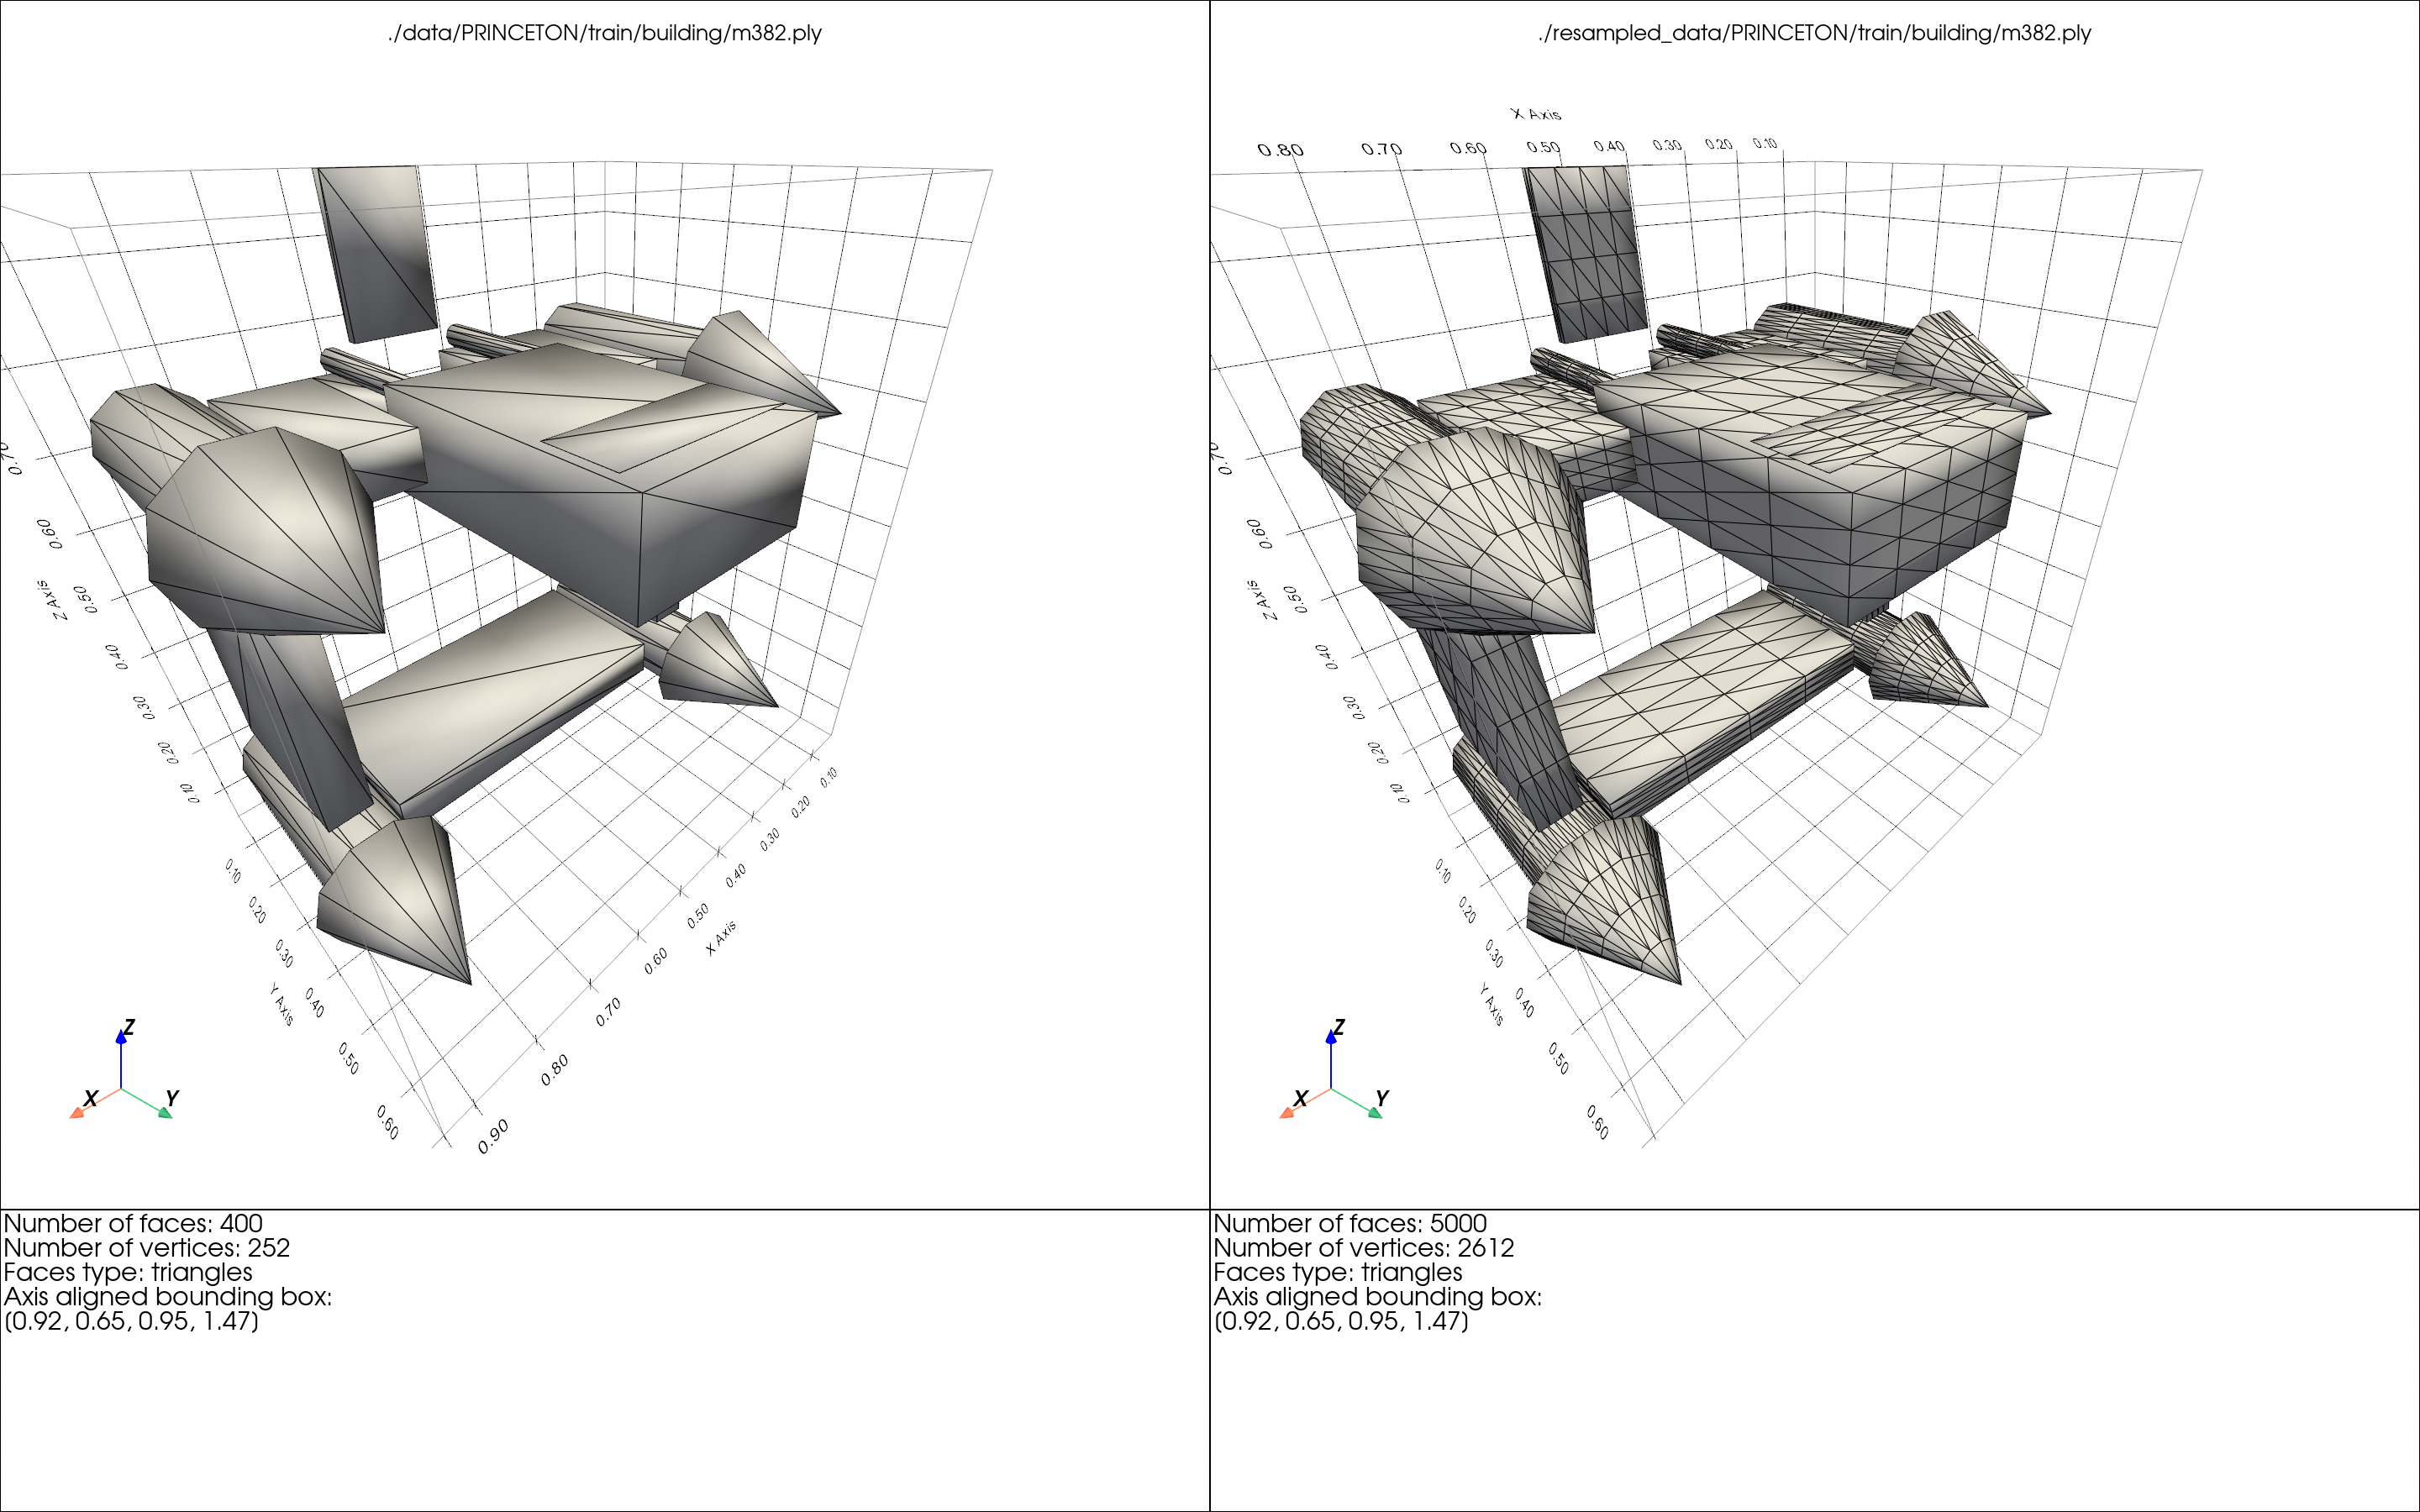
\includegraphics[width=\linewidth]
  {assets/preprocessing/resampling/castle_resampled.png}
  \caption{Comparison of the original 3D mesh of a castle on the left with its resulting super-sampled mesh on the right.}
  \label{fig:resampled_castle}
\end{figure}

\subsection{Normalizing Shapes}
Besides the remeshing of all 3D meshes, we also have to normalize the shapes.
This is very important because the some of the features we extract will be skewed, giving inconsistent results, if the
shapes are not normalized.
The normalization process consists of four steps, each of which is described in detail:
\begin{enumerate}
    \item Translating barycenter to the origin of the centre of the coordinate system
    \item Aligning the shape such as the major eigenvector corresponds to the $x$ axis, the medium corresponds to the $y$ axis and the minor to $z$ axis
    \item Flipping the shape such that the number of vertices at the positive side of each axis is greater than on the negative side
    \item Rescaling the shape to the unit cube
\end{enumerate}

We describe our shapes as meshes.
This is, a shape $\mathcal{S} = (V_{\mathcal{S}}, F_{\mathcal{S}})$, where $V_{\mathcal{S}} \in \mathbb{M}_{N,3}(\mathbb{R})$ and $F_{\mathcal{S}} \in \mathbb{M}_{M,3}(\mathbb{N})$.
We will describe each of these steps as a function of the vertices of a shape: $f_{TR},f_{AL},f_{FL},f_{RS}: \mathbb{M}_{N,3}(\mathbb{R}) \times \mathbb{M}_{M,3}(\mathbb{N}) \rightarrow \mathbb{M}_{N,3}(\mathbb{R}) \times \mathbb{M}_{M,3}(\mathbb{N})$.
The normalisation process then becomes a simple composition of these functions:
\begin{equation}
    \mathcal{S}_{norm} = f_{RS}(f_{FL}(f_{AL}(f_{TR} (\mathcal{S})))) 
\end{equation}

\subsubsection{Translation of the barycenter to the origin}
The shape is described by the vertices 3D coordinates $V_{\mathcal{S}} = 
\begin{pmatrix}
    v_{1,x} & v_{1,y} & v_{1,z} \\
    \vdots & \vdots & \vdots \\
    v_{N,x} & v_{N,y} & v_{N,z} \\
\end{pmatrix}$
The translation to the barycenter is done as follows:
\begin{enumerate}
    \item Compute the barycenter \ref{barycenter_not} of the shape by averaging all vertex locations weighted by their triangle surfaces.
    \item Apply the translation matrix $Tr =
        \begin{pmatrix}
        -b_{\mathcal{S},x} & 0 & 0 \\
        0 & -b_{\mathcal{S},y} & 0 \\
        0 & 0 & -b_{\mathcal{S},z} \\
        \end{pmatrix}$
to the matrix of vertices such that:
\begin{equation}
    f_{TR}(V_{\mathcal{S}}, \cdot) = ((Tr \cdot V_{\mathcal{S}}^T)^T, \cdot)
\end{equation}
This subtracts the barycenter coordinates from all vertices such that the whole shape is translated to a coordinate
system with the barycenter at its origin.
\end{enumerate}


\subsubsection{Aligning the shape eigenvectors to the axes of coordinates}
In order to align the shape along its principal axes (i.e.\ its eigenvectors), we first need to determine the
eigenvectors by performing a principal component analysis.
That is solving the equations:
\begin{equation}
    det(Cov(V_{\mathcal{S}}) - \lambda \cdot \mathbb{I}_N) = 0
\end{equation}
\begin{equation}
    Cov(V_{\mathcal{S}}) \cdot \overrightarrow{v_{\lambda}} = \lambda \cdot \overrightarrow{v_{\lambda}}
\end{equation}

This results in a set of 3 eigenvectors ($\overrightarrow{v_{\lambda_1}}, \overrightarrow{v_{\lambda_2}}, \overrightarrow{v_{\lambda_3}}$).
Observe that the covariance matrix is symmetric, thus, not only do the eigenvectors form a basis in the 3D space, but they are orthogonal to each other.
Therefore, we can simply align the coordinate axes to the eigenvectors by simply applying a rotation matrix to the set of vertices of the shape of interest.
We want all our shapes to be aligned such that the biggest spread is in the direction of the $x$ axis, the medium
spread in the direction of the $y$ axis, and the smallest in the direction of the $z$ axis.
Therefore, prior to constructing the rotation matrix, we do a rearrangement of the eigenvectors such that $\lambda_1 \geq \lambda_2 \geq \lambda_3$.
With this rearrangement, we can define the procedure of aligning to the coordinate axes as follows:
\begin{equation}
    f_{AL}(V_{\mathcal{S}}, \cdot) = ((Ro \cdot V_{\mathcal{S}}^T)^T, \cdot)    
\end{equation}
, where $Ro = \begin{pmatrix}
        v_{\lambda_1,x} & v_{\lambda_1,y} & v_{\lambda_1,z} \\
        v_{\lambda_2,x} & v_{\lambda_2,y} & v_{\lambda_2,z} \\
        v_{\lambda_3,x} & v_{\lambda_3,y} & v_{\lambda_3,z} \\
        \end{pmatrix}$ 
is the rotation matrix that we use for the alignment. 

\subsubsection{Flipping the shape on momentum}
We want to flip the shape with respect to the planes defined by $x=0$, $y=0$ and $z = 0$ such that the shape is more
concentrated in the subspaces $x > 0$, $y > 0$ and $z > 0$ than in the subspaces $x < 0$, $y < 0$ and $z < 0$ respectively.
For simplicity, suppose that we want the shape only to be more concentrated (i.e.\ have more mass) in the subspace $x>0$ than in $x < 0$.
A simple idea is to consider the number of vertices appertaining to each subspace and flip the shape w.r.t.\ the plane $x=0$ if there are more vertices in $x < 0$.
However, this approach would not be ideal.

Consider a case where we have a lot of small triangles faces in $x < 0$, and a few very big triangles in $x > 0$.
Obviously, we would like to flip the shape such that the mass is more in $x > 0 $, which is not the case if we would
only consider the vertex count in each subspace.

A better approach is to consider the centres of the triangles described by vertices instead and their coordinates.
This idea is incorporated in the descriptor $f_i$ (see Table \ref{tab:notations}).
We compute such a descriptor for each plane of interest, namely $f_x, f_y, f_z$.
Using the sign of these descriptors, we can determine whether the shape has to be flipped w.r.t.\ a
certain plane.
This is incorporated in the following formula:
\begin{equation}
    f_{FL}(V_{\mathcal{S}}, \cdot) = ((Fl \cdot V_{\mathcal{S}}^T)^T, \cdot)
\end{equation},
where $Fl = \begin{pmatrix}
    sign(f_x) & 0 & 0 \\
    0 & sign(f_y) & 0 \\
    0 & 0 & sign(f_z) \\
\end{pmatrix}$ is the flipping decision matrix.

\subsubsection{Rescale shape to unit cube}
Since 3D models can be rescaled, in our application, we do not care about the size of the shapes in our database.
So that this does not cause issues for us when we compute features, we want to standardize the size of all shapes.
We chose to rescale them relative to their unit cube.
To achieve this, we simply multiply each vertex by a rescaling factor \ref{rescale_not}.

\begin{equation}
    f_{RS}(V_{\mathcal{S}}, \cdot) = (\sigma_{unit}(S) \cdot V_{\mathcal{S}}, \cdot)
\end{equation}

\subsection{Preprocessing results}

\subsubsection{Resampling}
In order to test how well our resampling pipeline worked, we compute the distribution histograms of the number of
faces and vertices before and after processing our processing.

The results are shown in Figure \ref{fig:resampling-faces-vertices}.
After resampling, nearly all shapes have exactly $5000$ faces and $2500$ vertices.

\begin{figure}[H]
    \centering
    \begin{subfigure}[b]{0.45\textwidth}
        \centering
        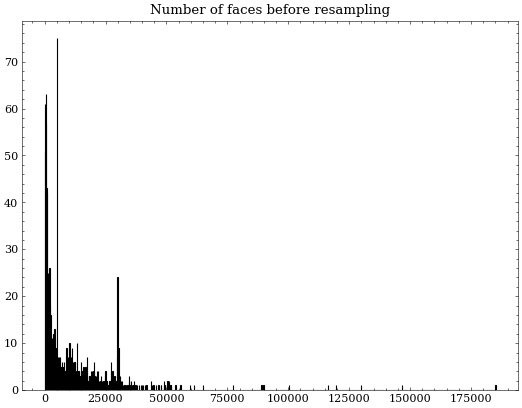
\includegraphics[width=\textwidth]{assets/preprocessing/Number_of_faces_before_resampling.png}
        \caption{Faces before resampling}
        \label{fig:resampling-faces-before}
    \end{subfigure}
    \hfill
    \begin{subfigure}[b]{0.45\textwidth}
        \centering
        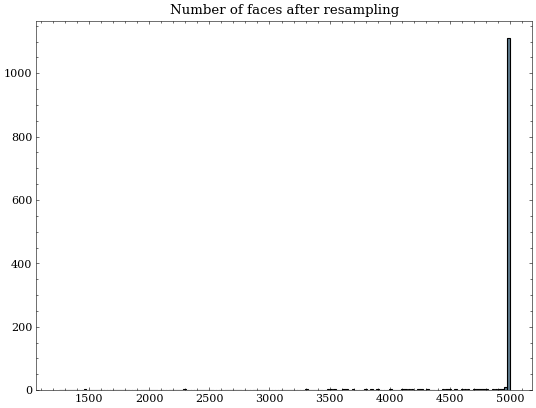
\includegraphics[width=\textwidth]{assets/preprocessing/Number_of_faces_after_resampling.png}
        \caption{Faces after resampling}
        \label{fig:resampling-faces-after}
    \end{subfigure}

\vspace{1cm}
    \begin{subfigure}[b]{0.45\textwidth}
        \centering
        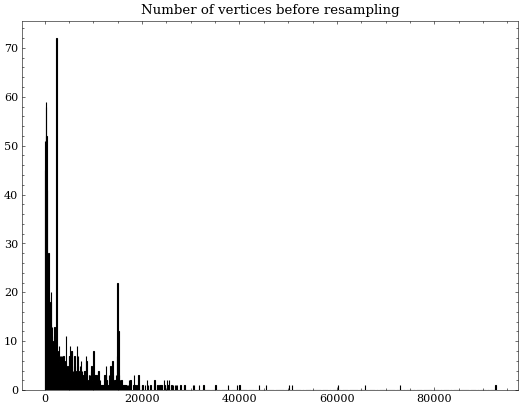
\includegraphics[width=\textwidth]{assets/preprocessing/Number_of_vertices_before_resampling.png}
        \caption{Vertices before resampling}
        \label{fig:resampling-vertices-before}
    \end{subfigure}
    \hfill
    \begin{subfigure}[b]{0.45\textwidth}
        \centering
        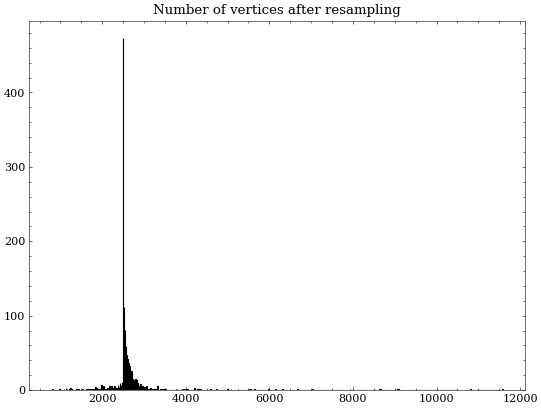
\includegraphics[width=\textwidth]{assets/preprocessing/Number_of_vertices_after_resampling.png}
        \caption{Vertices after resampling}
        \label{fig:resampling-vertices-after}
    \end{subfigure}
    \caption{Distribution of the number the number of faces \& vertices}
    \label{fig:resampling-faces-vertices}
\end{figure}

\subsubsection{Normalisation}
For testing the results of the normalisation, we compute histograms before and after, which we use to check some
pre-defined requirements regarding each step.

\paragraph{Centering}
In order to check that the barycenter of the shape is in the origin of the coordinate system, we compute the distance from the barycenter to the origin: $d(b_{\mathcal{S}}, (0,0,0))$.
For the processed - centered, shapes, we would expect the distance to be $0$.
We then plot a histogram to show the distribution of these distances, shown in Figure \ref{fig:resampling-barycenter}.

Before the normalisation, a small number of shapes have the barycenter far away from the origin (i.e.\ $d
($\ref{barycenter_not}$, (0,0,0)) \approx 3^{21}$.
After the normalisation, the biggest distance is approximately $0.002$.

The fact that we have a couple of shapes that deviate from our ideal distance is because of floating-point
approximations when computing the barycenter.
All in all, the results for this normalisation step are satisfying.

\begin{figure}[H]
    \centering
    \begin{subfigure}[b]{0.45\textwidth}
        \centering
        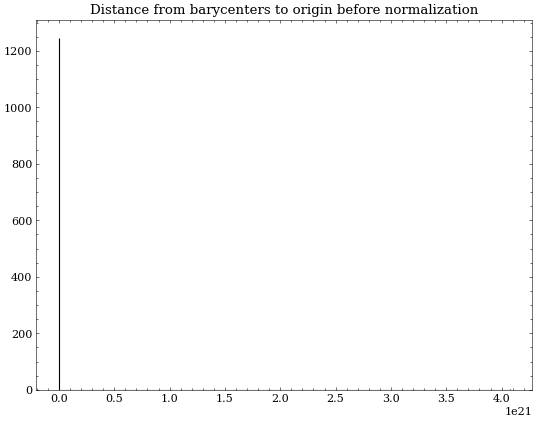
\includegraphics[width=\textwidth]{assets/preprocessing/Distance_from_barycenters_to_origin_before_normalization.png}
        \caption{Distance before normalisation}
        \label{fig:resampling-barycenter-before}
    \end{subfigure}
    \hfill
    \begin{subfigure}[b]{0.45\textwidth}
        \centering
        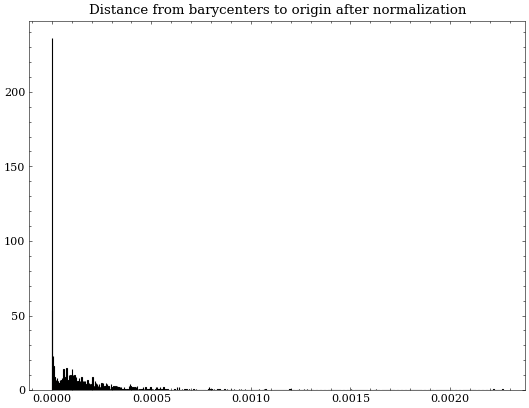
\includegraphics[width=\textwidth]{assets/preprocessing/Distance_from_barycenters_to_origin_after_normalization.png}
        \caption{Distance after normalisation}
        \label{fig:resampling-barycenter-after}
    \end{subfigure}
    \caption{Distribution of the distance from the barycenter to the origin}
    \label{fig:resampling-barycenter}
\end{figure}

\paragraph{Alignment}
After aligning to the principal component axes (i.e.\ eigenvectors), we expect the shape eigenvectors to be exactly equal to the coordinate axis vectors.

To test this, for each axis, we compute the distribution of the dot product of the corresponding eigenvector to that axis.
For instance, for the $x$-axis, we compute $ \overrightarrow{x} \cdot \overrightarrow{v_{\lambda_1}}$ where $\overrightarrow{x} = (1, 0, 0)$ and $\overrightarrow{v_{\lambda_1}}$ is the vector indicating the direction in which the shape have the maximal spread of the vertices.
The histograms from before and after this step can be seen in Figure \ref{fig:resampling-alignment}.
If the shapes are aligned correctly, this dot product should be equal to 1, since the angle should be 0.
This is what we observe in our histograms.

\begin{figure}[H]
    \centering
    \begin{subfigure}[b]{0.45\textwidth}
        \centering
        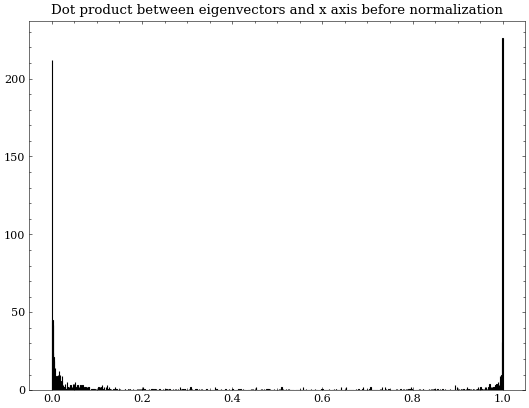
\includegraphics[width=\textwidth]{assets/preprocessing/Dot_product_between_eigenvectors_and_x_axis_before_normalization.png}
        \caption{Major eigenvector \& $x$ axis before normalisation}
        \label{fig:resampling-alignment-x-before}
    \end{subfigure}
    \hfill
    \begin{subfigure}[b]{0.45\textwidth}
        \centering
        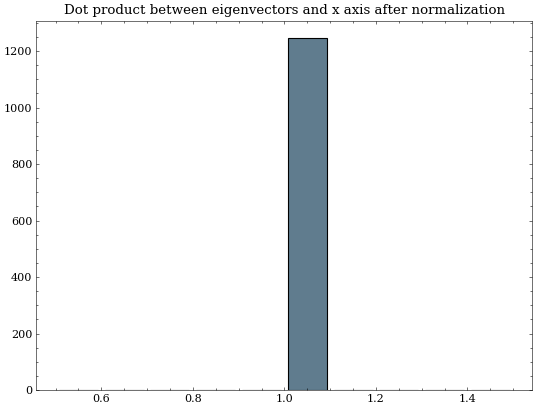
\includegraphics[width=\textwidth]{assets/preprocessing/Dot_product_between_eigenvectors_and_x_axis_after_normalization.png}
        \caption{Major eigenvector\& $x$ axis after normalisation}
        \label{fig:resampling-alignment-x-after}
    \end{subfigure}
    
\vspace{1cm}
    \begin{subfigure}[b]{0.45\textwidth}
        \centering
        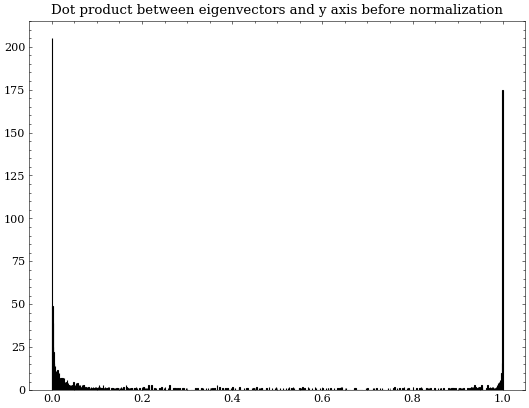
\includegraphics[width=\textwidth]{assets/preprocessing/Dot_product_between_eigenvectors_and_y_axis_before_normalization.png}
        \caption{Medium eigenvector \& $y$ axis before normalisation}
        \label{fig:resampling-alignment-y-before}
    \end{subfigure}
    \hfill
    \begin{subfigure}[b]{0.45\textwidth}
        \centering
        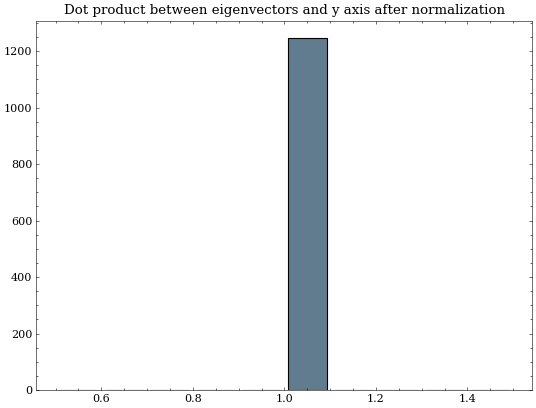
\includegraphics[width=\textwidth]{assets/preprocessing/Dot_product_between_eigenvectors_and_y_axis_after_normalization.png}
        \caption{Medium eigenvector \& $y$ axis after normalisation}
        \label{fig:resampling-alignment-y-after}
    \end{subfigure}

\vspace{1cm}
    \begin{subfigure}[b]{0.45\textwidth}
        \centering
        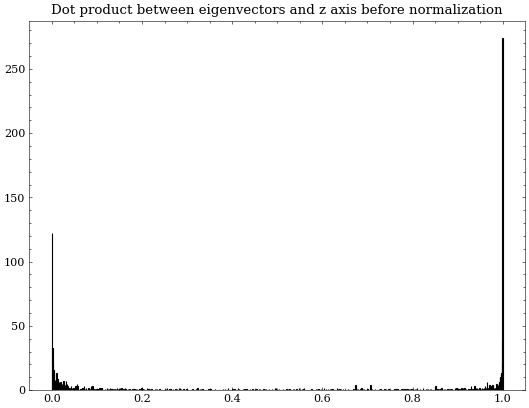
\includegraphics[width=\textwidth]{assets/preprocessing/Dot_product_between_eigenvectors_and_z_axis_before_normalization.png}
        \caption{Minor eigenvector \& $z$ axis before normalisation}
        \label{fig:resampling-alignment-z-before}
    \end{subfigure}
    \hfill
    \begin{subfigure}[b]{0.45\textwidth}
        \centering
        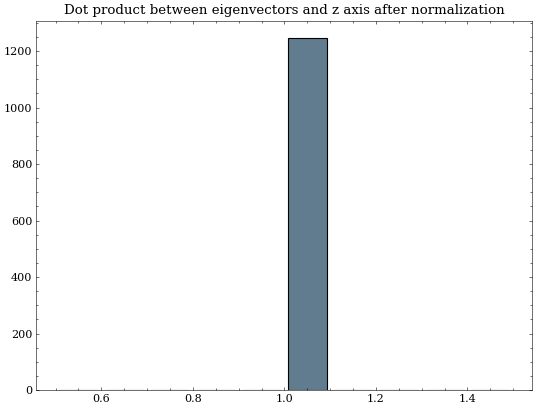
\includegraphics[width=\textwidth]{assets/preprocessing/Dot_product_between_eigenvectors_and_z_axis_after_normalization.png}
        \caption{Minor eigenvector \& $z$ axis after normalisation}
        \label{fig:resampling-alignment-z-after}
    \end{subfigure}
    \caption{Distribution of the dot product between an eigenvector and its respective coordinate axis}
    \label{fig:resampling-alignment}
\end{figure}


\paragraph{Flipping}
In a correctly implemented flipping step, we would expect the shape to have more mass on the positive side of
each plane $x = 0, y = 0, z = 0$.
We check whether this is the case by computing the flipping momentum components (i.e.\ \ref{flip_axis_not}) and
testing if they are positive.
If they are, then we flipped the shape correctly.

We calculate the weighted difference in the number of vertices on the positive and negative sides of $x = 0, y = 0, z
= 0$.
We plot the distributions before and after normalisation, shown in Figure \ref{fig:resampling-flipping}.
The histograms show that, after normalisation, we do have a positive difference - meaning, the flipping process is working as intended.

\begin{figure}[H]
    \centering
    \begin{subfigure}[b]{0.45\textwidth}
        \centering
        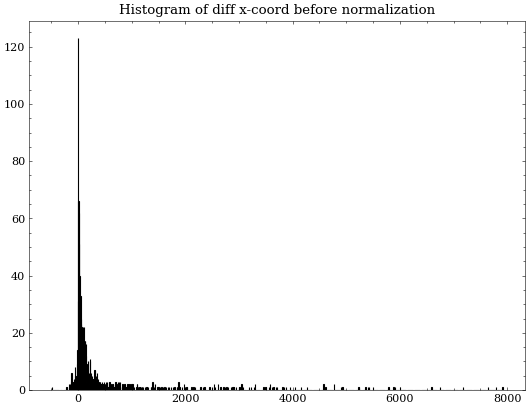
\includegraphics[width=\textwidth]{assets/preprocessing/Histogram_of_diff_x-coord_before_normalization.png}
        \caption{$x=0$ plane before normalisation}
        \label{fig:resampling-flipping-x-before}
    \end{subfigure}
    \hfill
    \begin{subfigure}[b]{0.45\textwidth}
        \centering
        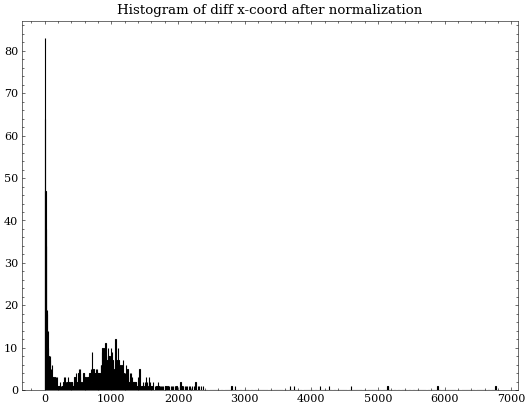
\includegraphics[width=\textwidth]{assets/preprocessing/Histogram_of_diff_x-coord_after_normalization.png}
        \caption{$x=0$ plane after normalisation}
        \label{fig:resampling-flipping-x-after}
    \end{subfigure}
    
\vspace{1cm}
    \begin{subfigure}[b]{0.45\textwidth}
        \centering
        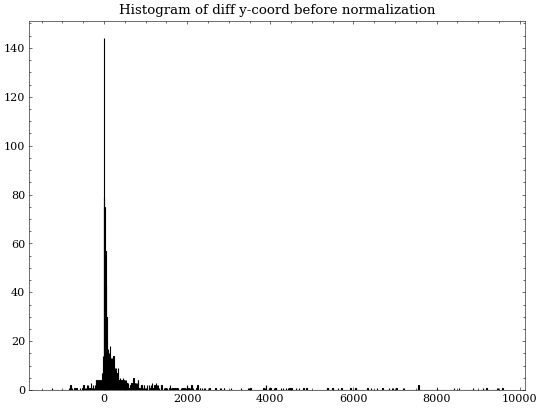
\includegraphics[width=\textwidth]{assets/preprocessing/Histogram_of_diff_y-coord_before_normalization.png}
        \caption{$y=0$ plane before normalisation}
        \label{fig:resampling-flipping-y-before}
    \end{subfigure}
    \hfill
    \begin{subfigure}[b]{0.45\textwidth}
        \centering
        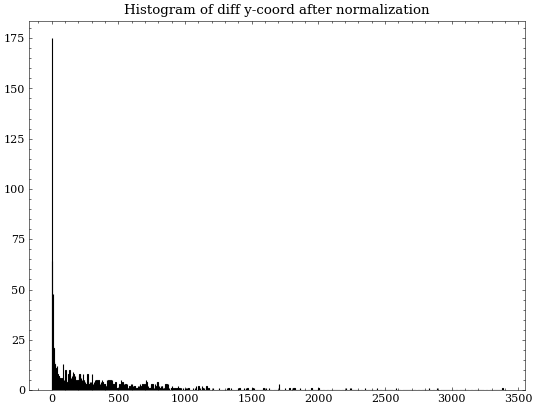
\includegraphics[width=\textwidth]{assets/preprocessing/Histogram_of_diff_y-coord_after_normalization.png}
        \caption{$y=0$ plane after normalisation}
        \label{fig:resampling-flipping-y-after}
    \end{subfigure}

\vspace{1cm}
    \begin{subfigure}[b]{0.45\textwidth}
        \centering
        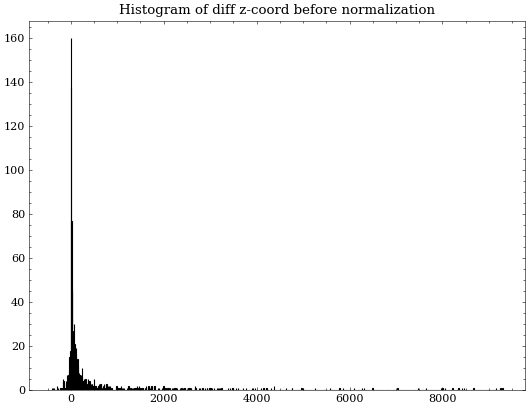
\includegraphics[width=\textwidth]{assets/preprocessing/Histogram_of_diff_z-coord_before_normalization.png}
        \caption{$z=0$ plane before normalisation}
        \label{fig:resampling-flipping-z-before}
    \end{subfigure}
    \hfill
    \begin{subfigure}[b]{0.45\textwidth}
        \centering
        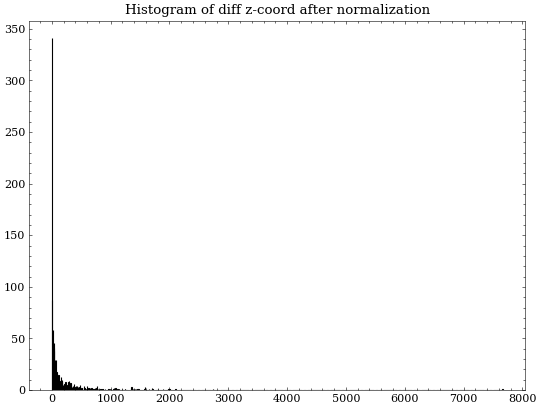
\includegraphics[width=\textwidth]{assets/preprocessing/Histogram_of_diff_z-coord_after_normalization.png}
        \caption{$z=0$ plane after normalisation}
        \label{fig:resampling-flipping-z-after}
    \end{subfigure}
    \caption{Distribution of the weighted difference of the number of vertices on the positive and negative sides of all axis planes}
    \label{fig:resampling-flipping}
\end{figure}


\paragraph{Scaling}
To check whether the shapes are rescaled correctly, we analyse the bounding box diagonal of the shape.
For a shape contained in the unit cube, the bounding box diagonal cannot be greater than $\sqrt{3} \approx 1.732$.

We plot the distribution of the diagonals before and after normalisation, shown in Figure \ref{fig:resampling-diagonal}.
After normalisation, all lengths are between $1$ and $1.73$, which is what we would expect for correctly rescaled shapes.

\begin{figure}[ht]
    \centering
    \begin{subfigure}[b]{0.45\textwidth}
        \centering
        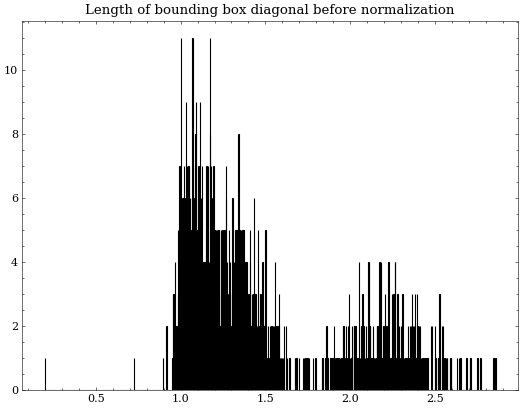
\includegraphics[width=\textwidth]{assets/preprocessing/Length_of_bounding_box_diagonal_before_normalization.png}
        \caption{Length before normalisation}
        \label{fig:resampling-diagonal-before}
    \end{subfigure}
    \hfill
    \begin{subfigure}[b]{0.45\textwidth}
        \centering
        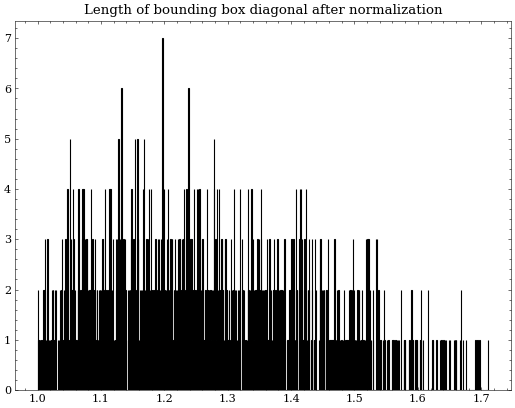
\includegraphics[width=\textwidth]{assets/preprocessing/Length_of_bounding_box_diagonal_after_normalization.png}
        \caption{Length after normalisation}
        \label{fig:resampling-diagonal-after}
    \end{subfigure}
    \caption{Distribution of the lengths of the bounding box diagonals}
    \label{fig:resampling-diagonal}
\end{figure}

\begin{figure}[ht]
    \centering
    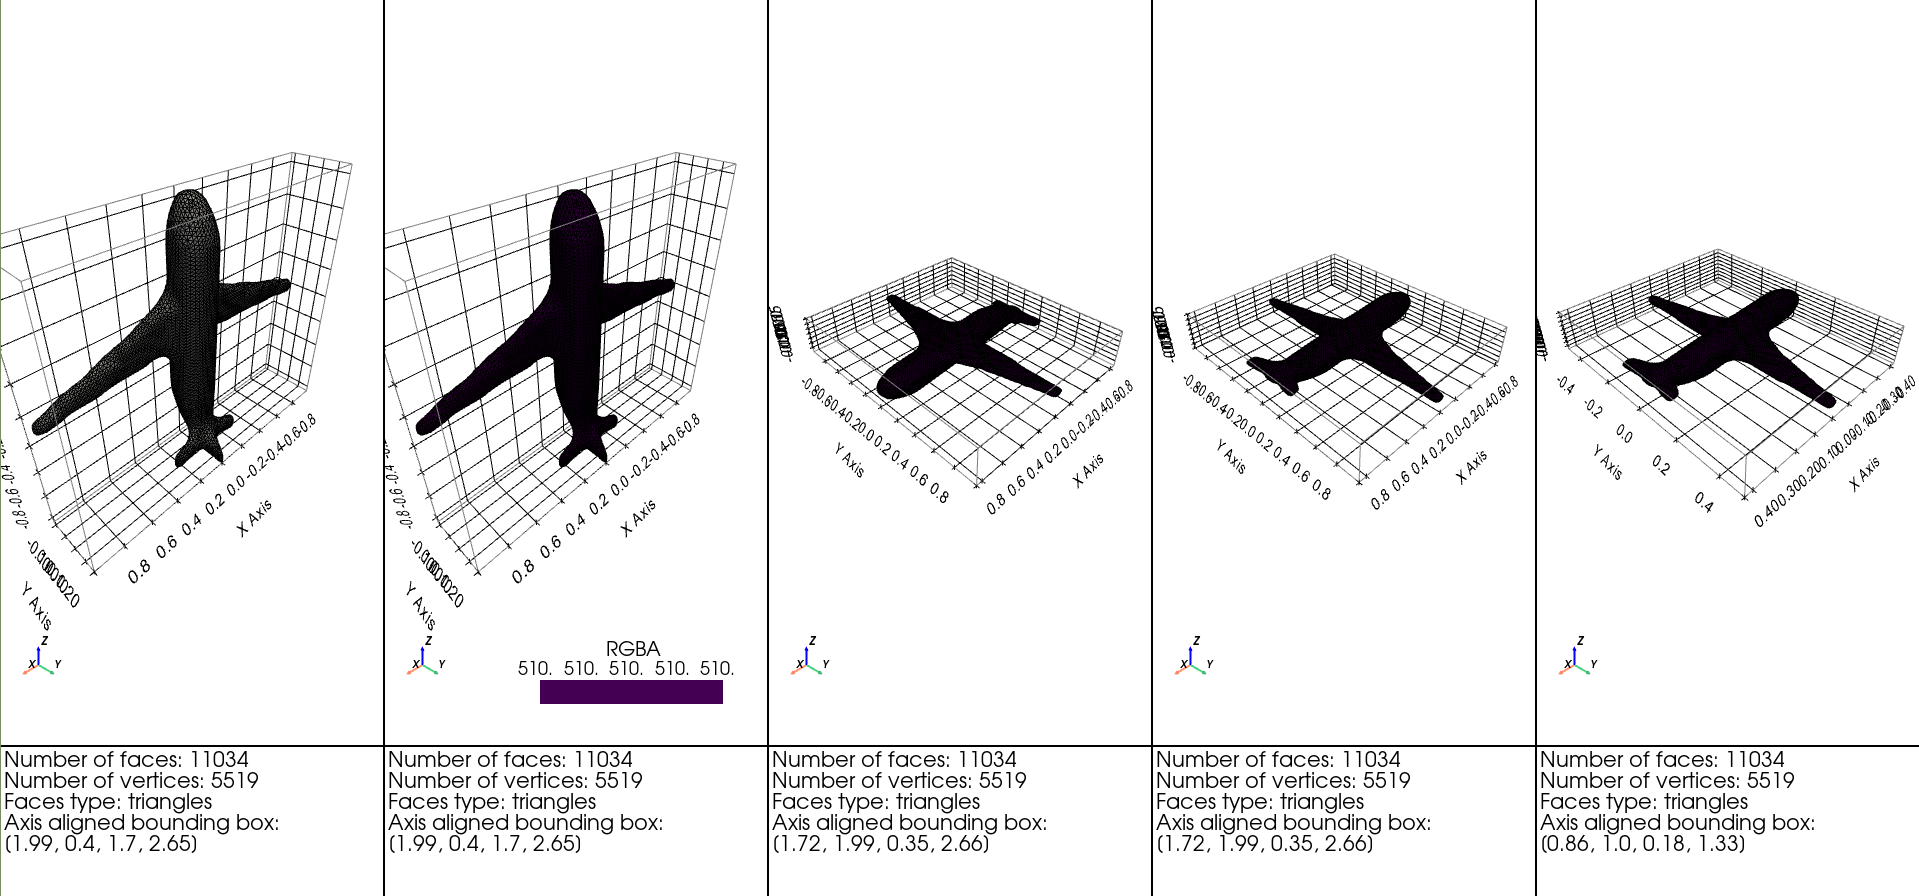
\includegraphics[width = 0.9\textwidth]{assets/visualisation/normalization_process.png}
    \caption{Normalisation process by steps}
    \label{fig:normalization-by-steps}
\end{figure}

Figure \ref{fig:normalization-by-steps} presents the step-by-step process of an airplane model going through
the normalization process.